\chapter{Research plan and progress}  
\section{First Year}
The first two months of the academic year were spent on reviewing the literature relevant to my research field, identifying the research gap and planning for my first study about identifying cognitive distortion on social media posts. The next six months were spent on drafting the annotation guideline, manually annotating the sample by myself and conducting the analysis. By the 8th month, the a conference paper based on the analysis was completed, but we decide to recruit students to relabel the task in order to validate my annotation. The next five months were spent on my second study about social support on reddit. I designed the study and collected data on the 9th month. From 10th - 12 months, I analysis the data and drafted a conference paper based on some of the findings. We submitted my second study to CHI 2019 at the 12th month. Then I spent the 13th month to prepare for the proposal presented in here and meanwhile working on my first study. 

\section{Second Year}
We are developing an annotation tool for the annotation of the cognitive distortion project. The annotation is expected to be completed on the 14th month, then I will redo the analysis and modify the draft of the paper. The cognitive distortion project focuses on monitoring valence (indicative of stress) and its interaction with vulnerability factors such as personality, satisfaction with life and self-disclosure level. The interaction between stress and vulnerability is an important underlying mechanism for the development of psychological disorders. Another objective of this study is to inspect whether cognitive distortion as a perpetuating mental health risk can be identified on social media. The cognitive distortion project is expected to be completed by the 15th month.

After that, we will extract the questions asked by the post author the social support study and cluster the questions according to their language attributes. The we will submit a short paper based on this analysis to another conference at the 16th month. On the 17th month, I am planning to expand the data from the previous reddit study by collect and analyzing posts from the same set of participants in other reddit communities. The aim of this study is to inspect whether people show more greater distress when disclosing a stressful life events endorse certain types of reddit communities and what are their language characteristics in various topics. We will analyze the topics, valence, language attributes and cognitive flexibility from the posts. This work is expected to be completed by 22th month. 

Then we will move on to the third project about chronic stress. Stressful events detection has been widely studied using social media data, whereas, chronic stress remains a research gap in this field. In the first stage, we intend to observe the characteristics from people who disclose a specific type of role stress on social media, such as being a care taker of children with autism. Then we compare their disclosure of chronic stress with those who suffer from a sudden stressful life events. The social support needs and support provided by the audiences will be characterized.

\section{Third Year}
In the second stage of the chronic stress project, we also inspect how people with strong or weak social ties disclose chronic stress on non-anonymous social media. Strong social ties have a buffering effect on stressful life experience. If strong ties are not available, people often seek support from the weak ties. We intend to compare the support provided by weak ties with those from strong ties. We will also observe the poster's interaction with the audiences. By inspecting how people with more strong ties maintain and develop social ties, we intend to provide insight for future design that help people to strengthen their social ties. The chronic stress study is expected to be finished on 26th months. 

The 27th - 31 months will be spent on cross-cultural studies. We will observe if there's any cultural differences in some of our previous findings. we intend to replicate some of the previous studies on a set of data from a Chinese forum called 'Tianya'. Then I will dedicate the rest of my PhD time on the dissertation \ref{fig:one}. 

% Figure
\begin{figure}
  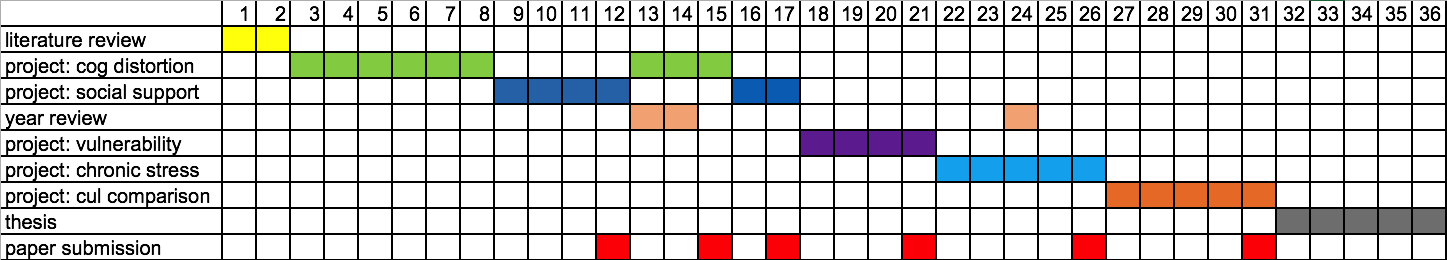
\includegraphics[width=160mm,scale=1.5]{Chapter5/timeline.png}
  \caption{PhD Timeline}
  \label{fig:one}
\end{figure}
